\subsection{Progettazione di dettaglio e codifica}
Questa fase comincia in seguito a quella precedente e termina con la \textit{Revisione di Qualifica}, ovvero dal 08-03-2020 al 02-04-2020.

\subsubsection{Attività}
\begin{itemize}
	\item \textbf{Incremento e verifica dei documenti}: realizzazione dell'\textit{Allegato Tecnico}, del \textit{Manuale utente} e del \textit{Manuale sviluppatore}. Inoltre, in caso di necessità, alcuni documenti verranno aggiornati;
	\item \textbf{Incremento e verifica delle attività}: viene ampliato lo studio delle tecnologie mancanti, necessarie per lo sviluppo del prodotto; 
	\item \textbf{\glo{Product Baseline}}: vengono realizzati i \textit{diagrammi delle classi}, che consentono di descrivere tipi di entità (con le loro caratteristiche e le eventuali relazioni), i \textit{diagrammi delle attività}, che permettono di descrivere i vari processi e i \textit{diagrammi di sequenza}. Inoltre verranno analizzati design patterns esistenti, con il fine di scegliere quello più adatto per il prodotto da creare.
	\item \textbf{\glo{Scrittura del codice e incrementi}}: viene realizzata la codifica, partendo dal \textit{Proof of Concept} già presente. Gli incrementi consistono nell'implementare sempre più casi d'uso, stabiliti nell'\textit{Analisi dei Requisiti}, iterando tra progettazione di dettaglio e realizzazione. La priorità sarà nei confronti di quelli obbligatori: in questo modo per ciascun caso d'uso, nell'eventualità di mancato completamento entro il periodo stabilito, è possibile attuare in sicurezza una ripianificazione dell'attività in questione.
	\begin{itemize}
	\item \textbf{Incremento I}: viene corretto il PoC in base alle segnalazioni ricevute dal proponente e in sede di Technology Baseline, viene studiata la libreria D3.js e vengono effettuate le dovute correzioni alla documentazione;
	
	\item \textbf{Incremento II}: viene studiata la libreria D3.js per individuare i parametri configurabili della visualizzazione Scatter Plot Matrix, e successivamente implementata nell'UI una sezione per permettere all'utente la personalizzazione di tale vista. Inizio stesura della documentazione da correlare al prodotto software\textbf{[UC6.1]};
	
	\item \textbf{Incremento III}: viene studiata la libreria D3.js per implementare la visualizzazione Heat Map e per individuare i relativi parametri configurabili, viene successivamente implementata nell'UI una sezione per permettere all'utente la personalizzazione di tale vista. Incremento della documentazione da correlare al prodotto software e incremento della documentazione per verifica e miglioramento continuo\textbf{[UC5.2, UC6.2]};
	
	\item \textbf{Incremento IV}: viene studiata la libreria D3.js per implementare la visualizzazione Force Field e per individuare i relativi parametri configurabili, viene successivamente implementata nell'UI una sezione per permettere all'utente la personalizzazione di tale vista. Incremento della documentazione da correlare al prodotto software e incremento della documentazione per verifica e miglioramento continuo\textbf{[UC5.3, UC6.3]};
	
	\item \textbf{Incremento V}: viene studiata la libreria D3.js per implementare la visualizzazione Proiezione Lineare Multi Asse e per individuare i relativi parametri configurabili, viene successivamente implementata nell'UI una sezione per permettere all'utente la personalizzazione di tale vista. Incremento della documentazione da correlare al prodotto software e incremento della documentazione per verifica e miglioramento continuo\textbf{[UC5.4, UC6.4]};
	
	\item \textbf{Incremento VI}: si pone l'attenzione nell'implementazione di un database già popolato e di una relativa sezione nell'UI in cui l'utente possa digitare una query per la selezione dei dati. Incremento della documentazione da correlare al prodotto software e incremento della documentazione per verifica e miglioramento continuo\textbf{[UC1.1.2]};
	
	\item \textbf{Incremento VII}: viene perfezionato il codice precedentemente scritto grazie alle correzioni ricevute durante la \textit{Technology Baseline} e dal proponente, e vengono verificati tutti i documenti precedentemente redatti.
	\end{itemize}
\end{itemize}

\subsubsection{Periodi}
La pianificazione di questa fase è stata organizzata nel modo seguente, in cui ad ogni periodo corrisponde lo sviluppo di un incremento:
\begin{itemize}
\item \textbf{Periodo 1}: \textit{(dal 08-03-2020 al 10-03-2020)} durante il primo periodo il gruppo si prepara alle attività di progettazione di dettaglio e codifica, inoltre vengono incrementanti i documenti per verifica e miglioramento continuo, al termine del periodo è fissata una milestone entro cui il gruppo dovrà aver terminato il primo incremento;

\item \textbf{Periodo 2}: \textit{(dal 10-03-2020 al 12-03-2020)} il secondo periodo ha una milestone fissata per il suo ultimo giorno, entro tale giorno dovrà essere completato il secondo incremento, dovrà essere iniziata la stesura dell'\textit{Allegato tecnico} e saranno scelti i design patterns più adatti per il prodotto;

\item \textbf{Periodo 3}: \textit{(dal 12-03-2020 al 16-03-2020)} il terzo periodo ha una milestone fissata per il suo ultimo giorno, entro tale giorno dovrà essere completato il terzo incremento;

\item \textbf{Periodo 4}: \textit{(dal 16-03-2020 al 20-03-2020)} il quarto periodo ha una milestone fissata per il suo ultimo giorno, entro tale giorno dovrà essere completato il quarto incremento e dovrà essere cominciata la stesura del \textit{Manuale utente} e del \textit{Manuale sviluppatore}, dovranno anche essere completati i diagrammi delle classi e i diagrammi delle attività;

\item \textbf{Periodo 5}: \textit{(dal 20-03-2020 al 25-03-2020)}: il quinto periodo ha una milestone fissata per il suo ultimo giorno, entro tale giorno dovrà essere completato il quinto incremento e dovranno essere completati i diagrammi di sequenza;

\item \textbf{Periodo 6}: \textit{(dal 25-03-2020 al 30-03-2020)}: il sesto periodo ha una milestone fissata per il suo ultimo giorno, entro tale giorno dovrà essere completato il sesto incremento;

\item \textbf{Periodo 7}: \textit{(dal 30-03-2020 al 02-04-2020)}: il settimo periodo ha una milestone fissata per il suo ultimo giorno, entro tale giorno dovrà essere completato il sesto incremento;

\end{itemize}

\subsubsection{Diagramma di Gantt: Progettazione di dettaglio e Codifica}
\begin{figure}[h]
 	\centering
	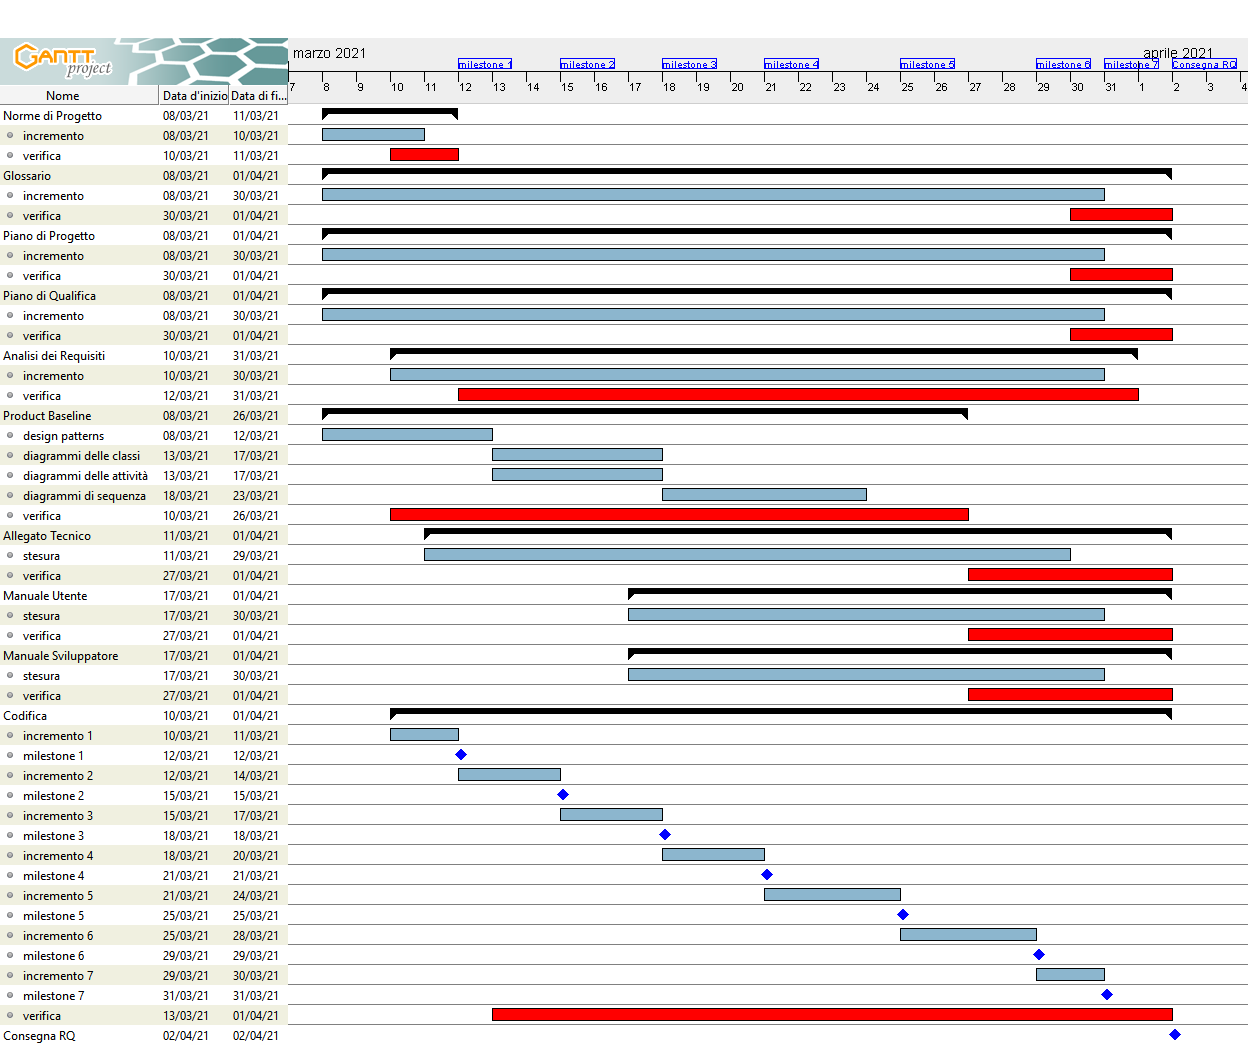
\includegraphics[scale=0.35]{Images/GanttPianificazioneProgettazioneDettaglioCodifica.png}
	\caption{Diagramma di Gantt dell'attività di Progettazione di dettaglio e Codifica}
\end{figure}
